\documentclass{article}
\usepackage{amsmath}
\usepackage{amssymb}
\usepackage{indentfirst}
\usepackage{bm}
\usepackage{graphicx}
\usepackage{geometry}
\geometry{left=2.5cm,right=2.5cm,top=2.5cm,bottom=2.5cm}

\title{8.511 Problem Set 4}
\author{Yijun Jiang}
%\email{yjjiang@mit.edu}
\date{\today}

\begin{document}
\maketitle
\section{Honeycomb Lattice}
\subsection{Part (a)}
The Bravais lattice vectors are
\begin{equation*}
	\mathbf{a}_1=\left(\frac{3}{2}a,\frac{\sqrt{3}}{2}a\right)\quad\quad\mathbf{a}_2=\left(0,\sqrt{3}a\right)
\end{equation*}

The basis vectors for the two carbon atoms are
\begin{equation*}
	\bm{\tau}_1=(0,0)\quad\quad\bm{\tau}_2=\left(0,\sqrt{3}a\right)
\end{equation*}

In order to make $\mathbf{a}_i\mathbf{b}_j=2\pi\delta_{ij}$, the reciprocal lattice vectors are
\begin{equation*}
	\mathbf{b}_1=\frac{4\pi}{3a}(1,0)\quad\quad\mathbf{b}_2=\frac{2\pi}{3a}\left(-1,\sqrt{3}\right)
\end{equation*}

The first Brillouin zone is drawned below.

~

~

~

\begin{figure}[!htbp]
	\centering
	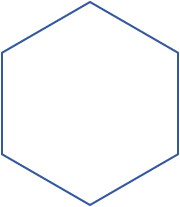
\includegraphics[width=2cm]{hex.png}\\
	\caption{The first Brillouin zone}
\end{figure}

\subsection{Part (b)}
The three nearest neighbors of $A$ are:
\begin{align*}
	B_1:\quad\bm{\mu}_1&=(a,0)\\
	B_2:\quad\bm{\mu}_2&=\left(-\frac{1}{2}a,\frac{\sqrt{3}}{2}a\right)\\
	B_3:\quad\bm{\mu}_3&=\left(-\frac{1}{2}a,-\frac{\sqrt{3}}{2}a\right)
\end{align*}

Then the off diagonal matrix element of $M_{\mathbf{k}}$ is
\begin{align*}
	M_{\mathbf{k},12}&=\langle\chi_{\mathbf{k}}^1|H|\chi_{\mathbf{k}}^2\rangle\\
	&=\frac{1}{N}\sum_{i,j}e^{-i\mathbf{k}\cdot\mathbf{R}_i}e^{i\mathbf{k}\cdot(\mathbf{R}_j+\bm{\tau}_2)}\langle\phi(\mathbf{r}-\mathbf{R}_i)|H|\phi(\mathbf{r}-(\mathbf{R}_j+\bm{\tau}_2))\rangle\\
	&=\frac{1}{N}e^{i\mathbf{k}\cdot\bm{\tau}_2}\sum_{i,j}e^{i\mathbf{k}\cdot(\mathbf{R}_j-\mathbf{R}_i)}\langle\phi(\mathbf{r})|H|\phi(\mathbf{r}-(\mathbf{R}_j-\mathbf{R}_i+\bm{\tau}_2))\\
	&=\frac{1}{N}e^{i\mathbf{k}\cdot\bm{\tau}_2}\sum_{i,j}\sum_{l=1}^3e^{i\mathbf{k}\cdot(\mathbf{R}_j-\mathbf{R}_i)}\langle\phi(\mathbf{r})|H|\phi(\mathbf{r}-(\mathbf{R}_j-\mathbf{R}_i+\bm{\tau}_2))\delta_{\bm{\mu}_l,\mathbf{R}_j-\mathbf{R}_i+\bm{\tau}_2}\\
	&=\frac{1}{N}e^{i\mathbf{k}\cdot\bm{\tau}_2}\sum_i\sum_{l=1}^3e^{i\mathbf{k}\cdot(\bm{\mu}_l-\bm{\tau}_2)}\langle\phi(\mathbf{r})|H|\phi(\mathbf{r}-\bm{\mu}_l)\rangle\\
	&=t\sum_{l=1}^3e^{i\mathbf{k}\cdot\bm{\mu}_i}\\
	&=t\left(e^{ik_xa}+e^{-i\frac{1}{2}k_xa+i\frac{\sqrt{3}}{2}k_ya}+e^{-i\frac{1}{2}k_xa-i\frac{\sqrt{3}}{2}k_ya}\right)\\
	&=t\left(\left(\cos k_xa+2\cos\frac{1}{2}k_xa\cos\frac{\sqrt{3}}{2}k_ya\right)+i\left(\sin k_xa-2\sin\frac{1}{2}k_xa\cos\frac{\sqrt{3}}{2}k_ya\right)\right)
\end{align*}

The diagonal entries vanish because the orbital energies are zero and they do not contain nearest neighbor coupling.

Therefore, the Schr\"{o}dinger equation can be written as
\begin{equation*}
	\left(\begin{array}{cc}0&t\displaystyle{\sum_{i=1}^3}e^{i\mathbf{k}\cdot\bm{\mu}_i}\\t\displaystyle{\sum_{i=1}^3}e^{-i\mathbf{k}\cdot\bm{\mu}_i}&0\end{array}\right)\left(\begin{array}{c}c_1\\c_2\end{array}\right)=E(\mathbf{k})\left(\begin{array}{c}c_1\\c_2\end{array}\right)
\end{equation*}
where the explicit form the of off-diagonal element is given above.

\subsection{Part (c)}
Solving this eigenvalue problem, we have
\begin{align*}
	E_\pm(\mathbf{k})&=\pm\left|t\sum_{i=1}^3e^{i\mathbf{k}\cdot\bm{\mu}_i}\right|\\
	&=\pm t\left(\left(\cos k_xa+2\cos\frac{1}{2}k_xa\cos\frac{\sqrt{3}}{2}k_ya\right)^2+\left(\sin k_xa-2\sin\frac{1}{2}k_xa\cos\frac{\sqrt{3}}{2}k_ya\right)^2\right)^{\frac{1}{2}}\\
	&=\pm t\sqrt{1+4\cos^2\frac{\sqrt{3}}{2}k_ya+4\cos\frac{3}{2}k_xa\cos\frac{\sqrt{3}}{2}k_ya}
\end{align*}

This dispersion relation is plotted in Fig.\ref{Dirac}. Dirac cones can be seen on the corners of the first (Wigner-Seitz) Brillouin zone.
\begin{figure}[!htbp]
	\centering
	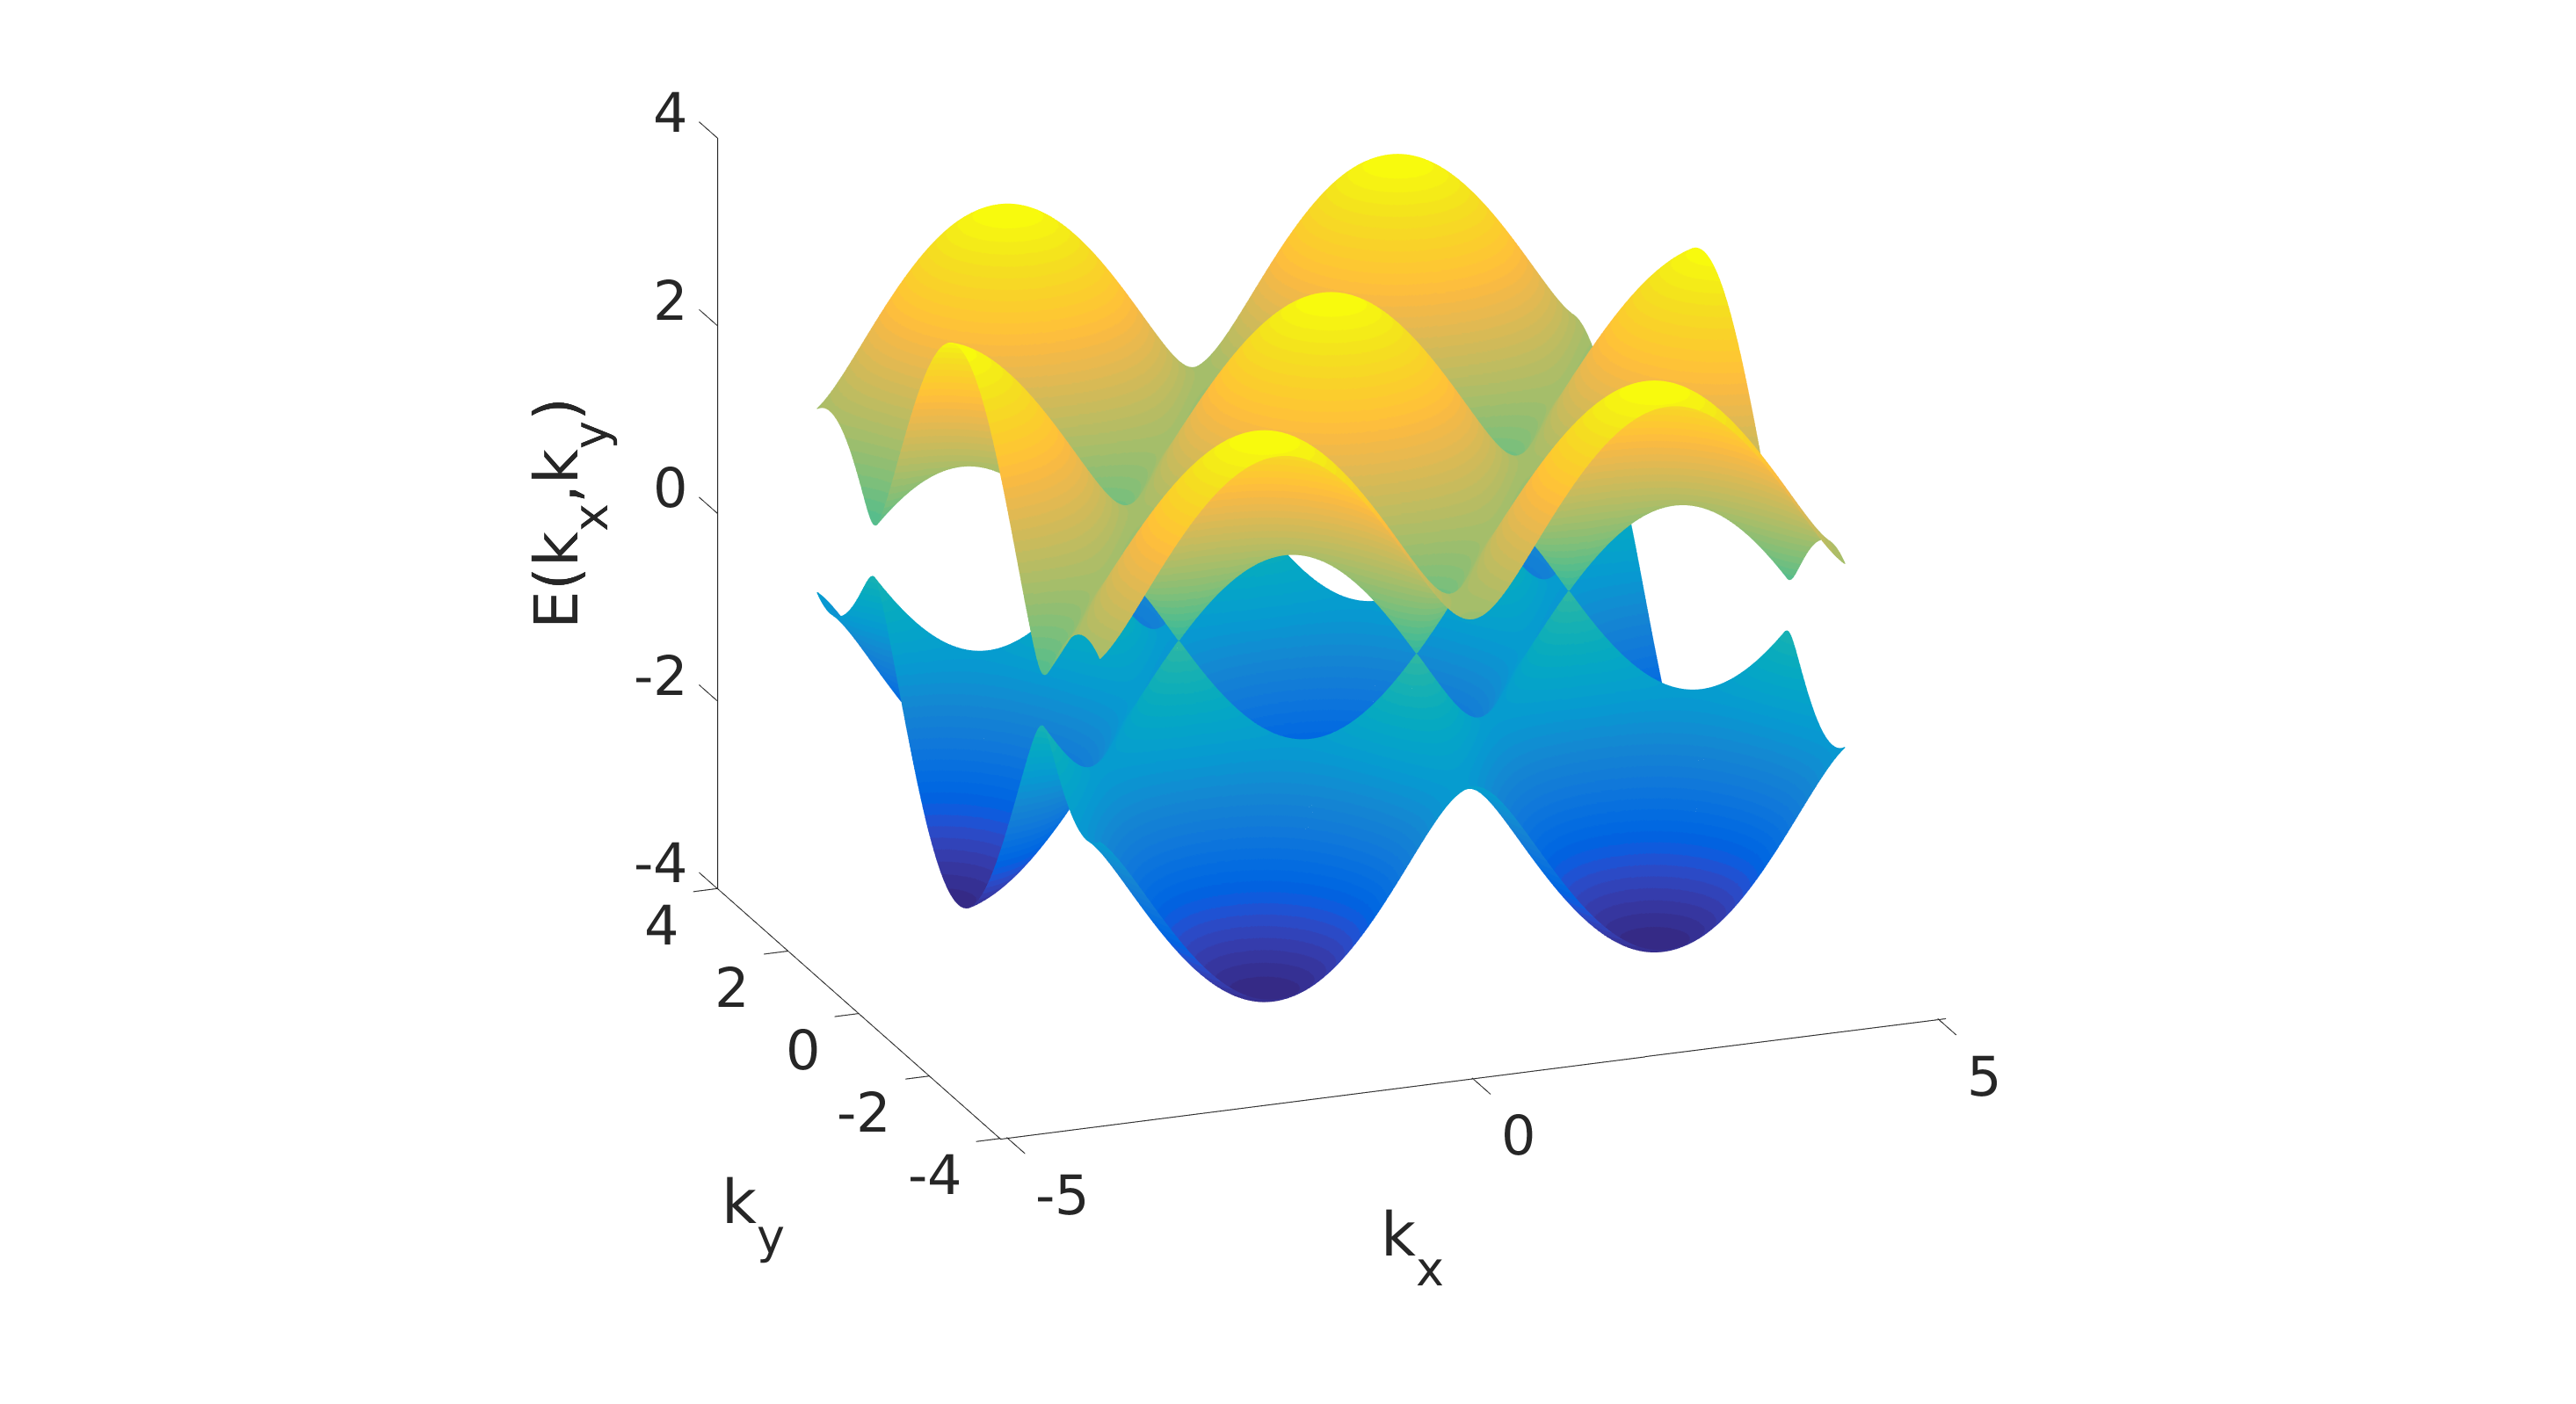
\includegraphics[width=12cm]{Dirac.eps}\\
	\caption{Dirac cones in the band structure of graphene}\label{Dirac}
\end{figure}

\section{Carbon Nanotubes}
\subsection{Part (a)}
From the previous section, we can write $E_\pm(\mathbf{k})$ as
\begin{equation}
	E_\pm(\mathbf{k})=\pm t\sqrt{\left(1+2\cos\frac{\sqrt{3}}{2}k_ya\right)^2+4\cos\frac{\sqrt{3}}{2}k_ya\left(\cos\frac{3}{2}k_xa-1\right)}\label{plus}
\end{equation}
or
\begin{equation}
	E_\pm(\mathbf{k})=\pm t\sqrt{\left(1-2\cos\frac{\sqrt{3}}{2}k_ya\right)^2+4\cos\frac{\sqrt{3}}{2}k_ya\left(\cos\frac{3}{2}k_xa+1\right)}\label{minus}
\end{equation}

Then it is easy to see that the Brillouin zone corners have $E_\pm(\mathbf{k})=0$. These corners are
\begin{equation*}
	\frac{2\pi}{a}\left(0,\pm\frac{2\sqrt{3}}{9}\right)\quad\quad\frac{2\pi}{a}\left(\pm\frac{1}{3},\pm\frac{\sqrt{3}}{9}\right)
\end{equation*}

It suffices to prove the linear dispersion at two of the six corners, namely $\frac{2\pi}{a}\left(0,\frac{2\sqrt{3}}{9}\right)$ and $\frac{2\pi}{a}\left(\frac{1}{3},\frac{\sqrt{3}}{9}\right)$.

Let $\mathbf{K}=\frac{2\pi}{a}\left(0,\frac{2\sqrt{3}}{9}\right)$, and $\mathbf{k}=\mathbf{K}+(\delta k_x,\delta k_y)$, where $\delta k_x,\delta k_y\ll\frac{2\pi}{a}$.

Plugging into equation (\ref{plus}), we get
\begin{align*}
	E_\pm(\mathbf{k})&=\pm t\sqrt{\left(1+2\cos\left(\frac{2\pi}{3}+\frac{\sqrt{3}}{2}\delta k_ya\right)\right)^2+4\cos\left(\frac{2\pi}{3}+\frac{\sqrt{3}}{2}\delta k_ya\right)\left(\cos\frac{3}{2}\delta k_xa-1\right)}\\
	&\approx\pm t\sqrt{\left(\frac{3}{2}\delta k_xa\right)^2+\left(\frac{3}{2}\delta k_ya\right)^2}\\
	&=\pm\frac{3ta}{2}|\mathbf{k}-\mathbf{K}|
\end{align*}

Let $\mathbf{K}=\frac{2\pi}{a}\left(\frac{1}{3},\frac{\sqrt{3}}{9}\right)$, and $\mathbf{k}=\mathbf{K}+(\delta k_x,\delta k_y)$, where $\delta k_x,\delta k_y\ll\frac{2\pi}{a}$.

Plugging into equation (\ref{minus}), we get
\begin{align*}
	E_\pm(\mathbf{k})&=\pm t\sqrt{\left(1-2\cos\left(\frac{\pi}{3}+\frac{\sqrt{3}}{2}\delta k_ya\right)\right)^2+4\cos\left(\frac{\pi}{3}+\frac{\sqrt{3}}{2}\delta k_ya\right)\left(\cos\left(\pi+\frac{3}{2}\delta k_xa\right)+1\right)}\\
	&\approx\pm t\sqrt{\left(\frac{3}{2}\delta k_xa\right)^2+\left(\frac{3}{2}\delta k_ya\right)^2}\\
	&=\pm\frac{3ta}{2}|\mathbf{k}-\mathbf{K}|
\end{align*}

Therefore, near the Briliouin zone corners, we have $E_\pm(\mathbf{k})\approx\pm\frac{3ta}{2}|\mathbf{k}-\mathbf{K}|$.

\subsection{Part (b)}
The location of Dirac cones forms a honeycomb lattice in the reciprocal space. Therefore, these Dirac cones can be classified into two inequivalent classes. A Dirac cone is inequivalent to its nearest neighboring Dirac cones.

Each $p_z$ orbital contributes one electron. Therefore, each unit cell has two valence electrons. So the lowest band is completely filled. The Fermi level is located at the top of $E_-(\mathbf{k})$, which is also the bottom of $E_+(\mathbf{k})$. This is exactly the energy at the Dirac cones, which, according to the calculation above, equals zero. Thus, $E_F=0$.


Notice that there are two Dirac cones in the first Brillouin zone. Another factor of $2$ comes from spin degeneracy. Then for the upper band we have
\begin{align*}
	N(E)&=2\times 2\times\int_{\textup{1st B.z.}}\frac{d\mathbf{k}}{(2\pi)^2}\delta\left(E-\frac{3ta}{2}|\mathbf{k}-\mathbf{K}|\right)\\
	&=\frac{2}{3\pi^2ta}\int_{\textup{1st B.z.}}k\delta\left(k-\frac{2E}{3ta}\right)dkd\theta\\
	&=\frac{8E}{9\pi t^2a^2}
\end{align*}

The lower band gives the same result. At the Fermi surface, $N(E_F)=0$.

\subsection{Part (c)}
In an armchair tube, the wavefunction satisfies periodic condition
\begin{equation*}
	\phi(\mathbf{r})=\phi(\mathbf{r}+3N_xa\hat{\mathbf{x}})
\end{equation*}
where $N_x$ is the number of periods along the tube circumference.

According to Bloch theorem, this means a restriction on $k_x$.
\begin{align*}
	&e^{3iN_xk_xa}=1\\
	&k_x=\frac{2\pi n_x}{3N_xa}
\end{align*}
where $n_x\in\mathbb{Z}$.

Similarly, in a zigzag tube, the wavefunction satisfies periodic condition
\begin{equation*}
	\phi(\mathbf{r})=\phi(\mathbf{r}+\sqrt{3}N_ya\hat{\mathbf{y}})
\end{equation*}
where $N_y$ is the number of periods along the tube circumference.

According to Bloch theorem, this means a restriction on $k_y$.
\begin{align*}
	&e^{\sqrt{3}iN_yk_ya}=1\\
	&k_y=\frac{2\pi n_y}{3N_ya}
\end{align*}
where $n_y\in\mathbb{Z}$.

These lines are drawn in Fig.\ref{lines}.
\begin{figure}[!htbp]
	\centering
	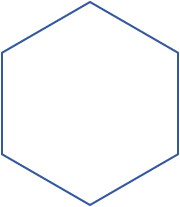
\includegraphics[width=3cm]{hex.png}\quad\quad\quad\quad\quad\quad\quad\quad\quad\quad\quad\quad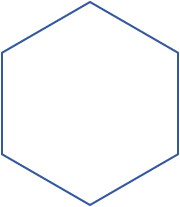
\includegraphics[width=3cm]{hex.png}\\
	\caption{Restrictions on $\mathbf{k}$ in two kinds of carbon nanotubes (left: armchair; right: zigzag)}\label{lines}
\end{figure}

\subsection{Part (d)}
When $\frac{n_x}{N_x}\in\mathbb{Z}$, the line passes right through Dirac cones. Therefore, the bottom of the upper band touches the top of the lower band at $E_F=0$. Thus the system is metallic.

All such lines are equivalent. One example is when $n_x=0$. Then $k_x=0$. Plugging in $E_\pm(\mathbf{k})$ we have
\begin{align*}
E_-(k_y)&=t\min\left(1-2\cos\frac{\sqrt{3}}{2}k_ya,1+2\cos\frac{\sqrt{3}}{2}k_ya\right)\\
E_+(k_y)&=t\max\left(1-2\cos\frac{\sqrt{3}}{2}k_ya,1+2\cos\frac{\sqrt{3}}{2}k_ya\right)
\end{align*}

Fig.\ref{armchair} shows the two bands.
\begin{figure}[!htbp]
	\centering
	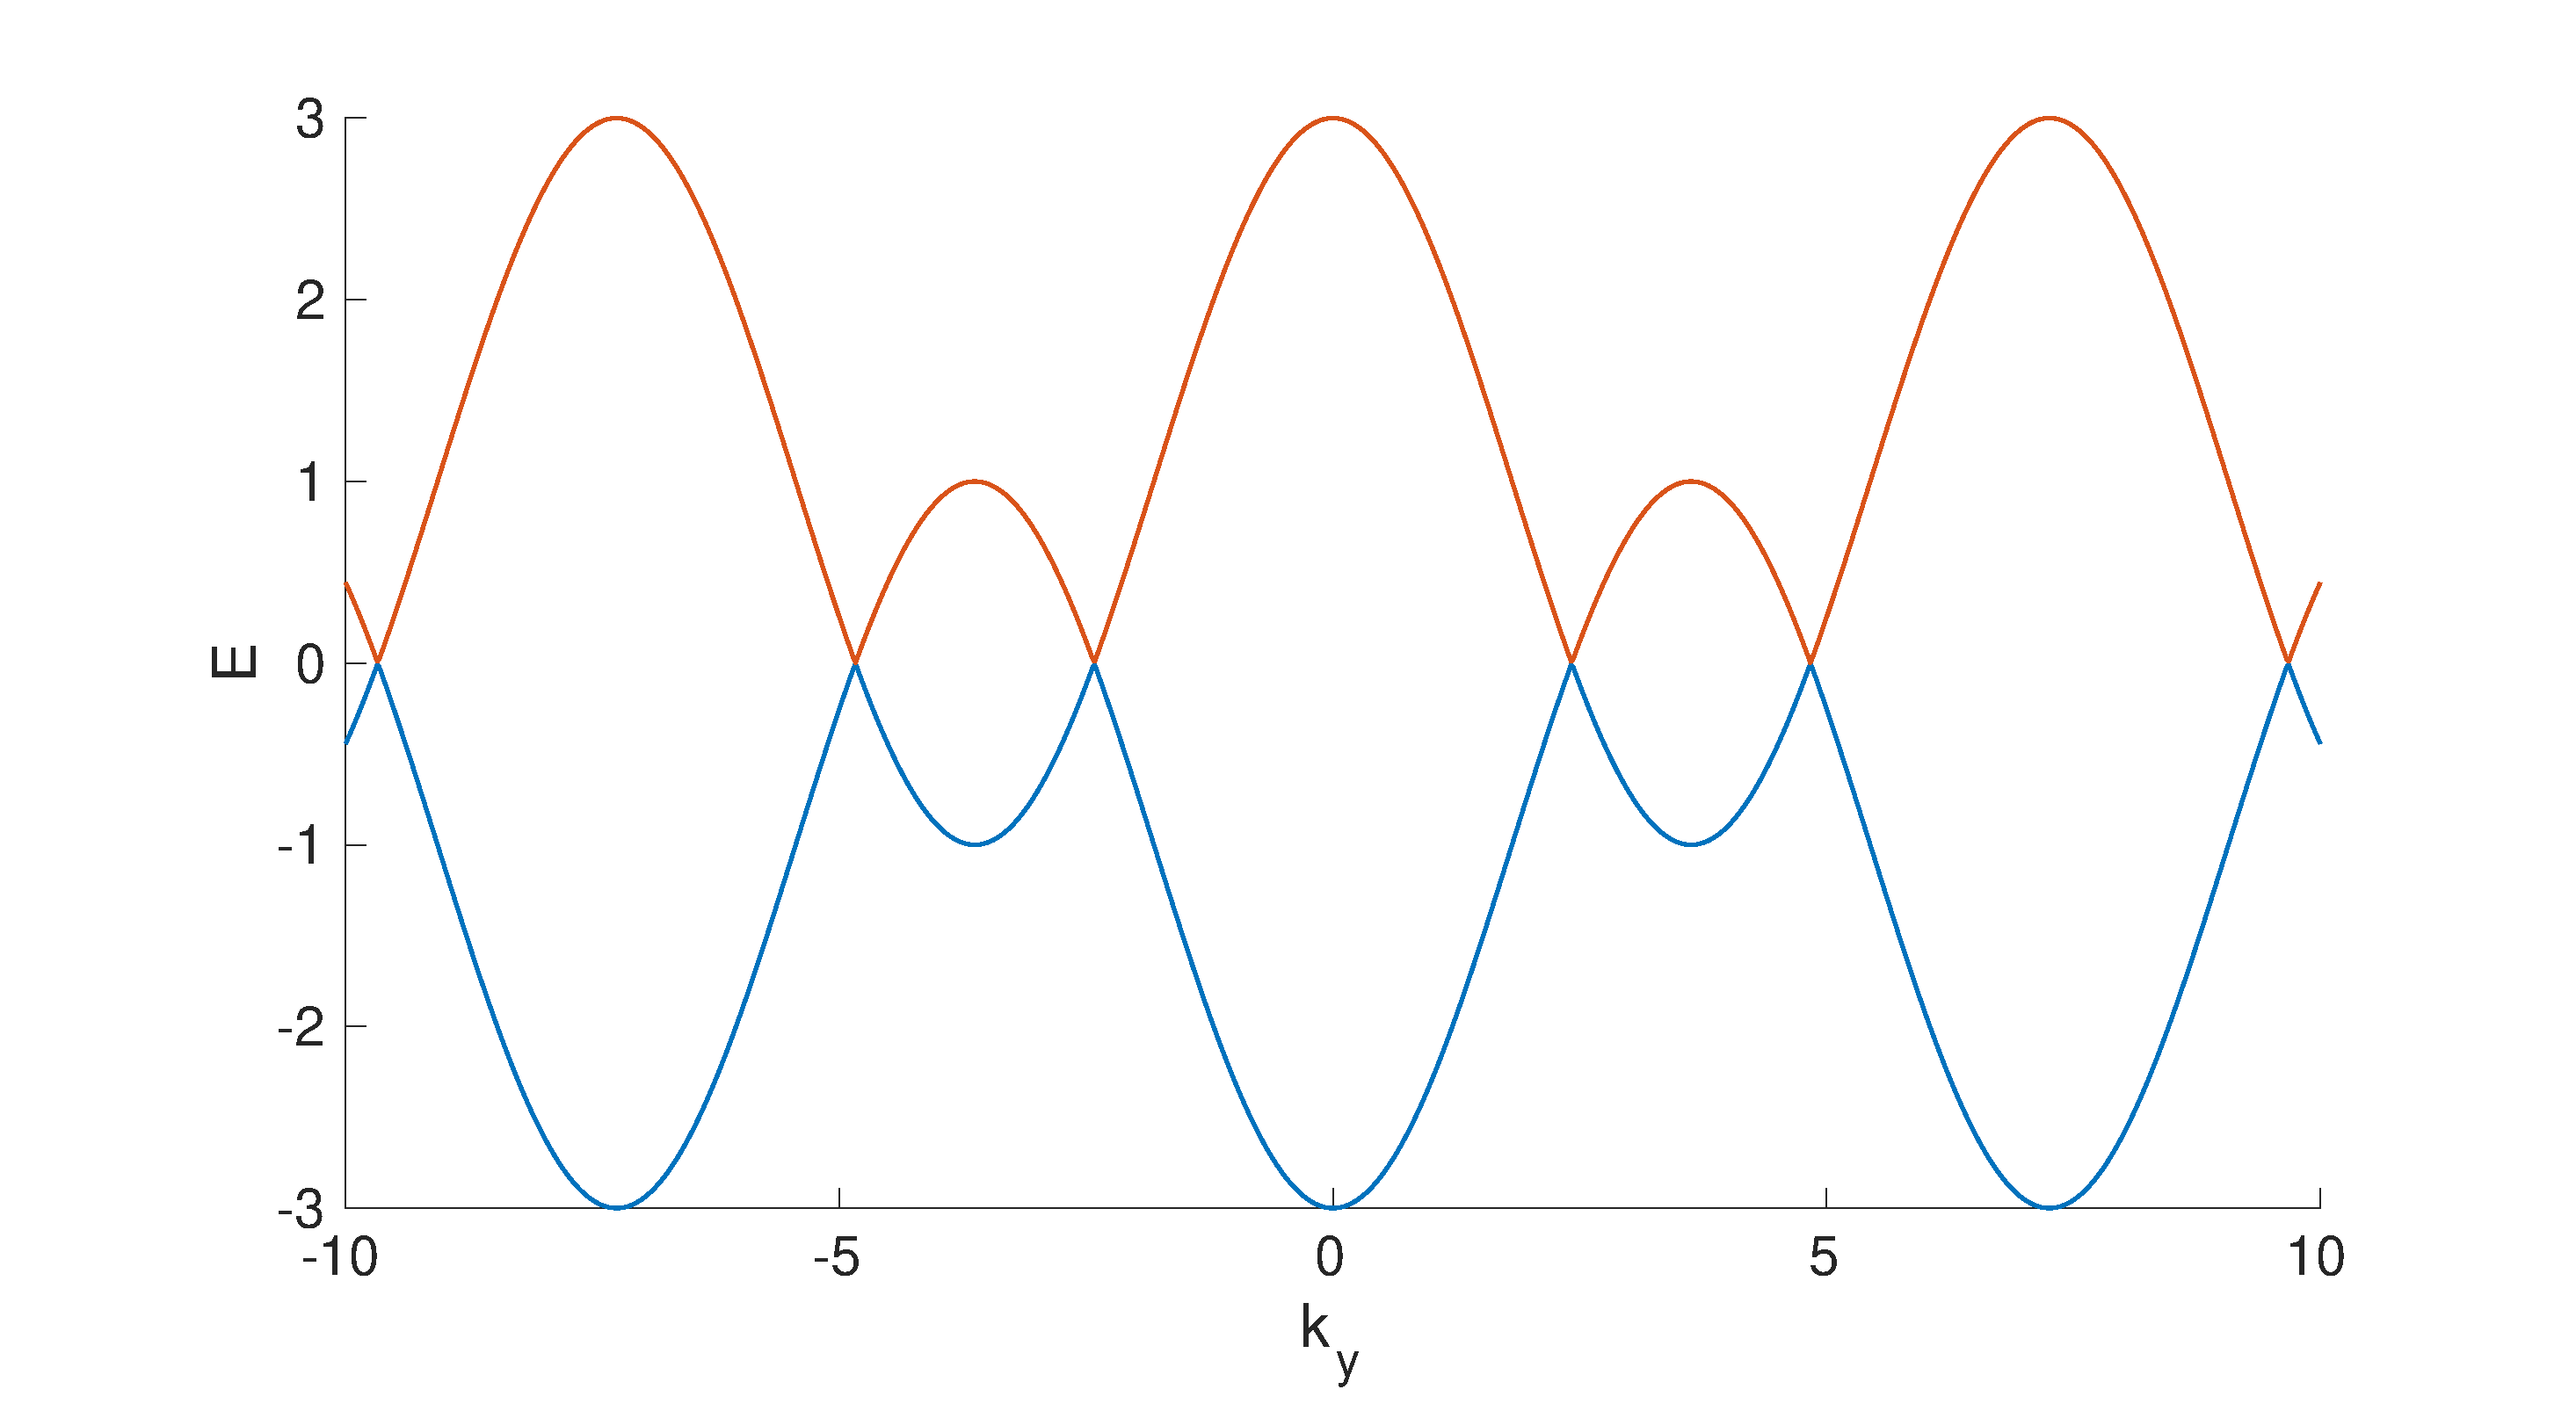
\includegraphics[width=12cm]{armchair.eps}\\
	\caption{Band structure of the armchair tube}\label{armchair}
\end{figure}

The line periodically passes through a first-type Dirac cone and then a second-type Dirac cone. Thus over a period of $\frac{4\pi}{\sqrt{3}a}$ there are two cones. Another factor of $2$ comes from spin degeneracy. Close to the Dirac points, the dispersion is $E_\pm(k_y)\approx\frac{3ta}{2}|k_y-K_y|$. DOS of the upper band near Fermi surface is thus (same result for the lower band)
\begin{align*}
	N_a(E)&=2\times 2\times\int_{\textup{1st B.z.}}\frac{dk_y}{2\pi}\delta\left(E-\frac{3ta}{2}|k_y-K_y|\right)\\
	&=\frac{4}{3\pi ta}\int_{\textup{1st B.z.}}\delta\left(k_y-\frac{2E}{3ta}\right)dk_y\\
	&=\frac{4}{3\pi ta}
\end{align*}

\subsection{Part (e)}
In the metallic case, the line for the zigzag tube must also pass through some Dirac points. Therefore,
\begin{equation*}
\frac{2\pi n_y}{\sqrt{3}N_ya}=\frac{2\pi}{3\sqrt{3}a}\textup{ or }\frac{4\pi}{3\sqrt{3}a}\quad\quad\textup{for some $n_y$}
\end{equation*}

In other words,
\begin{equation*}
n_y=\frac{2}{3}N_y\textup{ or }\frac{4}{3}N_y
\end{equation*}

So $N_y$, the number of periods along the circumference, must be a multiple of $3$. If $N_y$ is a large multiple of $3$ plus a small remainder, the line can be very close to some Dirac points, producing some small band gaps that enable semiconducting. For example, let $N_y=31$ and $n_y=20$. Then $k_y=\frac{40\pi}{31\sqrt{3}}a\approx\frac{4\pi}{3\sqrt{3}a}$. Fig.\ref{zigzag} shows this case.
\begin{figure}[!htbp]
	\centering
	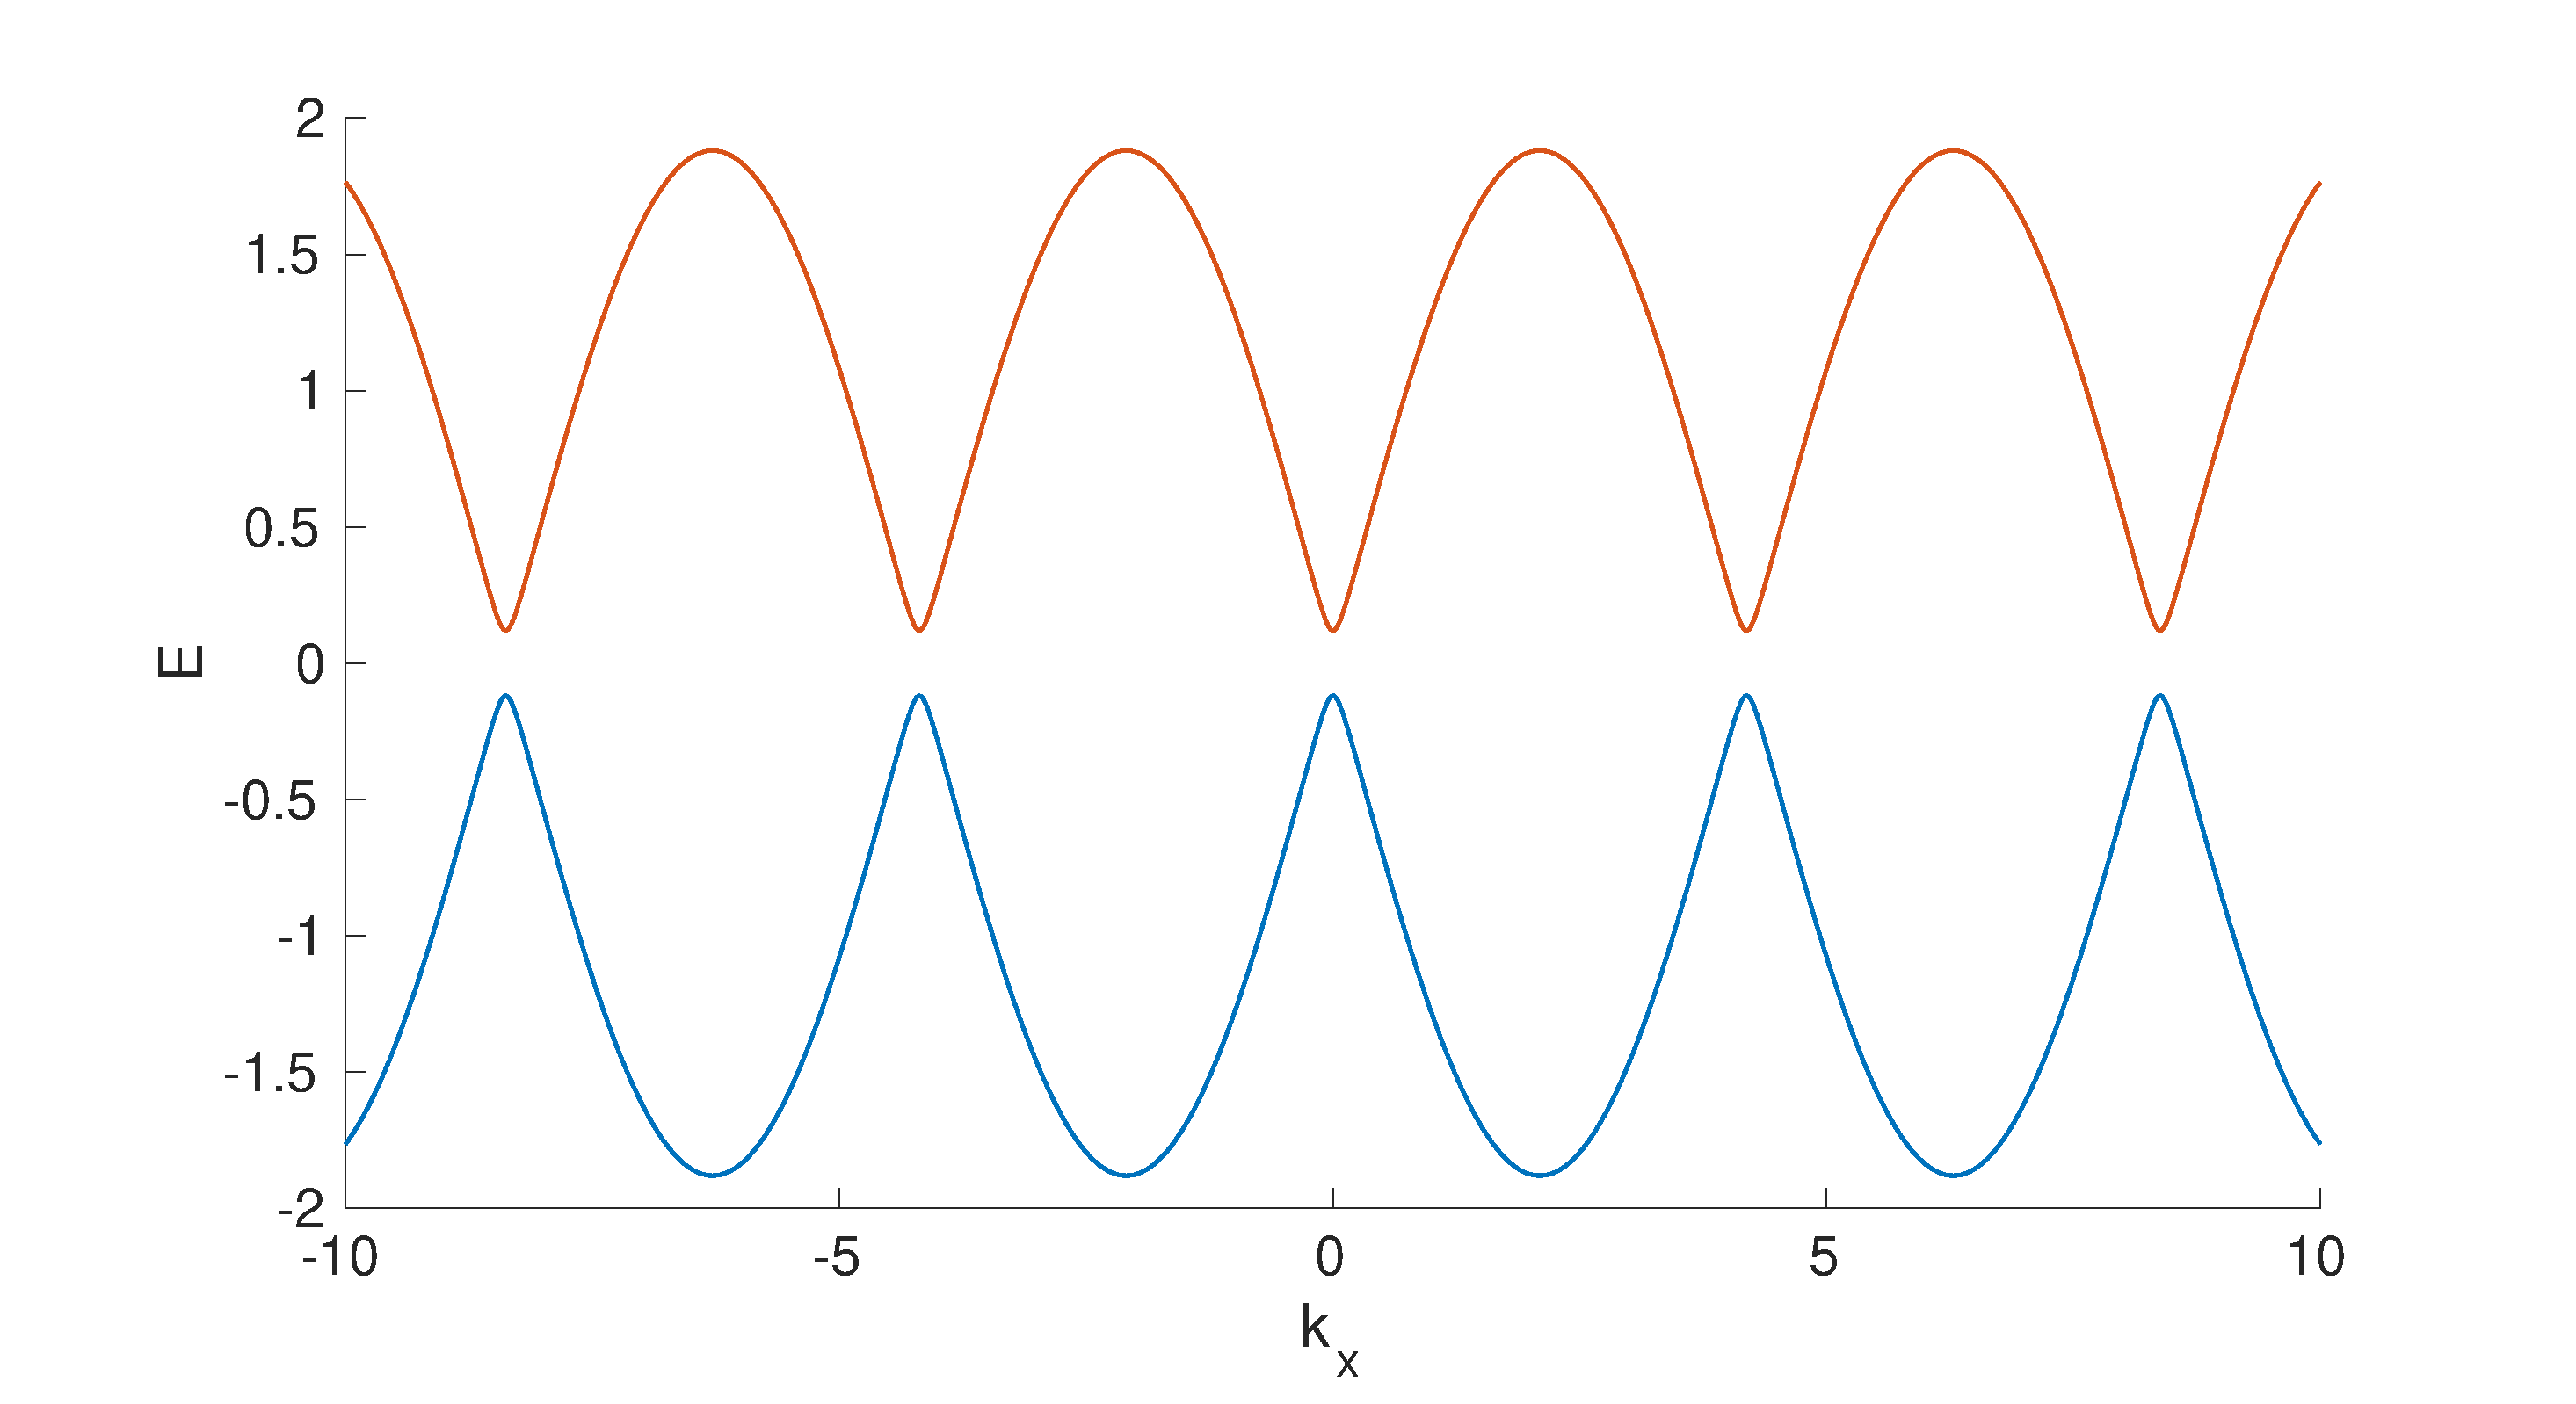
\includegraphics[width=12cm]{zigzag.eps}\\
	\caption{Band structure of the semiconducting zigzag tube}\label{zigzag}
\end{figure}

In the metallic case, notice that the line only passes through one equivalent class of Dirac points. So we conclude that DOS near the Fermi energy will be only one half of the armchair case.
\begin{equation*}
	N_z(E)=\frac{1}{2}N_a(E)=\frac{2}{3\pi ta}
\end{equation*}

\end{document}
